% Options for packages loaded elsewhere
% Options for packages loaded elsewhere
\PassOptionsToPackage{unicode}{hyperref}
\PassOptionsToPackage{hyphens}{url}
\PassOptionsToPackage{dvipsnames,svgnames,x11names}{xcolor}
%
\documentclass[
  letterpaper,
  DIV=11,
  numbers=noendperiod]{scrartcl}
\usepackage{xcolor}
\usepackage[top=2cm,bottom=2.5cm,left=2cm,right=2cm]{geometry}
\usepackage{amsmath,amssymb}
\setcounter{secnumdepth}{-\maxdimen} % remove section numbering
\usepackage{iftex}
\ifPDFTeX
  \usepackage[T1]{fontenc}
  \usepackage[utf8]{inputenc}
  \usepackage{textcomp} % provide euro and other symbols
\else % if luatex or xetex
  \usepackage{unicode-math} % this also loads fontspec
  \defaultfontfeatures{Scale=MatchLowercase}
  \defaultfontfeatures[\rmfamily]{Ligatures=TeX,Scale=1}
\fi
\usepackage{lmodern}
\ifPDFTeX\else
  % xetex/luatex font selection
\fi
% Use upquote if available, for straight quotes in verbatim environments
\IfFileExists{upquote.sty}{\usepackage{upquote}}{}
\IfFileExists{microtype.sty}{% use microtype if available
  \usepackage[]{microtype}
  \UseMicrotypeSet[protrusion]{basicmath} % disable protrusion for tt fonts
}{}
\makeatletter
\@ifundefined{KOMAClassName}{% if non-KOMA class
  \IfFileExists{parskip.sty}{%
    \usepackage{parskip}
  }{% else
    \setlength{\parindent}{0pt}
    \setlength{\parskip}{6pt plus 2pt minus 1pt}}
}{% if KOMA class
  \KOMAoptions{parskip=half}}
\makeatother
% Make \paragraph and \subparagraph free-standing
\makeatletter
\ifx\paragraph\undefined\else
  \let\oldparagraph\paragraph
  \renewcommand{\paragraph}{
    \@ifstar
      \xxxParagraphStar
      \xxxParagraphNoStar
  }
  \newcommand{\xxxParagraphStar}[1]{\oldparagraph*{#1}\mbox{}}
  \newcommand{\xxxParagraphNoStar}[1]{\oldparagraph{#1}\mbox{}}
\fi
\ifx\subparagraph\undefined\else
  \let\oldsubparagraph\subparagraph
  \renewcommand{\subparagraph}{
    \@ifstar
      \xxxSubParagraphStar
      \xxxSubParagraphNoStar
  }
  \newcommand{\xxxSubParagraphStar}[1]{\oldsubparagraph*{#1}\mbox{}}
  \newcommand{\xxxSubParagraphNoStar}[1]{\oldsubparagraph{#1}\mbox{}}
\fi
\makeatother


\usepackage{longtable,booktabs,array}
\newcounter{none} % for unnumbered tables
\usepackage{calc} % for calculating minipage widths
% Correct order of tables after \paragraph or \subparagraph
\usepackage{etoolbox}
\makeatletter
\patchcmd\longtable{\par}{\if@noskipsec\mbox{}\fi\par}{}{}
\makeatother
% Allow footnotes in longtable head/foot
\IfFileExists{footnotehyper.sty}{\usepackage{footnotehyper}}{\usepackage{footnote}}
\makesavenoteenv{longtable}
\usepackage{graphicx}
\makeatletter
\newsavebox\pandoc@box
\newcommand*\pandocbounded[1]{% scales image to fit in text height/width
  \sbox\pandoc@box{#1}%
  \Gscale@div\@tempa{\textheight}{\dimexpr\ht\pandoc@box+\dp\pandoc@box\relax}%
  \Gscale@div\@tempb{\linewidth}{\wd\pandoc@box}%
  \ifdim\@tempb\p@<\@tempa\p@\let\@tempa\@tempb\fi% select the smaller of both
  \ifdim\@tempa\p@<\p@\scalebox{\@tempa}{\usebox\pandoc@box}%
  \else\usebox{\pandoc@box}%
  \fi%
}
% Set default figure placement to htbp
\def\fps@figure{htbp}
\makeatother





\setlength{\emergencystretch}{3em} % prevent overfull lines

\providecommand{\tightlist}{%
  \setlength{\itemsep}{0pt}\setlength{\parskip}{0pt}}



 


\usepackage{booktabs}
\usepackage{longtable}
\usepackage{array}
\usepackage{multirow}
\usepackage{wrapfig}
\usepackage{float}
\usepackage{colortbl}
\usepackage{pdflscape}
\usepackage{tabularx}
\usepackage{xltabular}
\usepackage{threeparttable}
\usepackage{threeparttablex}
\usepackage[normalem]{ulem}
\usepackage{makecell}
\usepackage{xcolor}
\usepackage{caption}
\usepackage{float}
\usepackage{chngcntr}
\usepackage{arydshln}
\renewcommand{\arraystretch}{1.35}
\floatplacement{table}{H}
\floatplacement{figure}{H}
\newcounter{parentfig}
\renewcommand{\thefigure}{D.\arabic{figure}}
\renewcommand{\thetable}{D.\arabic{table}}
\captionsetup{format=plain, indention=0pt}
\KOMAoption{captions}{tableheading}
\makeatletter
\@ifpackageloaded{caption}{}{\usepackage{caption}}
\AtBeginDocument{%
\ifdefined\contentsname
  \renewcommand*\contentsname{Table of contents}
\else
  \newcommand\contentsname{Table of contents}
\fi
\ifdefined\listfigurename
  \renewcommand*\listfigurename{List of Figures}
\else
  \newcommand\listfigurename{List of Figures}
\fi
\ifdefined\listtablename
  \renewcommand*\listtablename{List of Tables}
\else
  \newcommand\listtablename{List of Tables}
\fi
\ifdefined\figurename
  \renewcommand*\figurename{Figure}
\else
  \newcommand\figurename{Figure}
\fi
\ifdefined\tablename
  \renewcommand*\tablename{Table}
\else
  \newcommand\tablename{Table}
\fi
}
\@ifpackageloaded{float}{}{\usepackage{float}}
\floatstyle{ruled}
\@ifundefined{c@chapter}{\newfloat{codelisting}{h}{lop}}{\newfloat{codelisting}{h}{lop}[chapter]}
\floatname{codelisting}{Listing}
\newcommand*\listoflistings{\listof{codelisting}{List of Listings}}
\makeatother
\makeatletter
\makeatother
\makeatletter
\@ifpackageloaded{caption}{}{\usepackage{caption}}
\@ifpackageloaded{subcaption}{}{\usepackage{subcaption}}
\makeatother
\usepackage{bookmark}
\IfFileExists{xurl.sty}{\usepackage{xurl}}{} % add URL line breaks if available
\urlstyle{same}
\hypersetup{
  pdftitle={Appendix D - Beagle Marine Park Data Analysis Report (stereo BRUV)},
  colorlinks=true,
  linkcolor={blue},
  filecolor={Maroon},
  citecolor={Blue},
  urlcolor={Blue},
  pdfcreator={LaTeX via pandoc}}


\title{Appendix D - Beagle Marine Park Data Analysis Report (stereo
BRUV)}
\usepackage{etoolbox}
\makeatletter
\providecommand{\subtitle}[1]{% add subtitle to \maketitle
  \apptocmd{\@title}{\par {\large #1 \par}}{}{}
}
\makeatother
\subtitle{South-east Marine Parks Network}
\author{}
\date{}
\begin{document}
\maketitle

\renewcommand*\contentsname{Table of contents}
{
\setcounter{tocdepth}{3}
\tableofcontents
}

\section{Data Analysis}\label{data-analysis}

Statistical methods and model selection results underpinning the natural
values reported in Appendix A.

\newpage{}

\subsection{Benthic ecosystem extent}\label{benthic-ecosystem-extent}

\begingroup\fontsize{10}{12}\selectfont

\begin{longtable}[t]{>{\raggedright\arraybackslash}m{2.41cm}>{\centering\arraybackslash}m{5.121cm}>{\centering\arraybackslash}m{1.807cm}>{\centering\arraybackslash}m{1.807cm}>{\centering\arraybackslash}m{2.109cm}>{\centering\arraybackslash}m{1.807cm}}

\caption{\label{tbl-c1-1}Habitat model selection results. Top
generalised additive models (GAMs) for predicting the probability of
occurrence of key habitats from full subset analyses. Differences
between the lowest reported corrected Akaike Information Criterion
(\(\Delta\)AICc), AICc weight (\(\omega\)AICc), variance explained
(R\(^2\)) and effective degrees of freedom (EDF) are reported for model
comparison. Model selection was based on the most parsimonious model
(fewest variables - shown in bold) within two units of the lowest AICc.}

\tabularnewline

\toprule
\cellcolor{gray!25}{\textbf{Response}} & \cellcolor{gray!25}{\textbf{Model}} & \cellcolor{gray!25}{\textbf{$\Delta$ AICc}} & \cellcolor{gray!25}{\textbf{$\omega$ AICc}} & \cellcolor{gray!25}{\textbf{$R^2$}} & \cellcolor{gray!25}{\textbf{EDF}}\\
\midrule
\endfirsthead
\multicolumn{6}{@{}l}{\textit{(continued)}}\\
\toprule
\cellcolor{gray!25}{\textbf{Response}} & \cellcolor{gray!25}{\textbf{Model}} & \cellcolor{gray!25}{\textbf{$\Delta$ AICc}} & \cellcolor{gray!25}{\textbf{$\omega$ AICc}} & \cellcolor{gray!25}{\textbf{$R^2$}} & \cellcolor{gray!25}{\textbf{EDF}}\\
\midrule
\endhead

\endfoot
\bottomrule
\endlastfoot
\textbf{Sand} & \textbf{detrended+roughness+aspect+year} & \textbf{0} & \textbf{0.423} & \textbf{0.05575} & \textbf{10.45}\\
\textbf{} & \textbf{detrended+roughness+aspect+year} & \textbf{0.878} & \textbf{0.273} & \textbf{0.05641} & \textbf{11.75}\\
\textbf{} & \textbf{detrended+roughness+aspect+year} & \textbf{1.238} & \textbf{0.228} & \textbf{0.05511} & \textbf{10.19}\\
\noalign{\arrayrulecolor{gray}}\cdashline{1-6}\noalign{\arrayrulecolor{black}}
\textbf{Sessile invertebrates} & \textbf{detrended+roughness+aspect+year} & \textbf{0} & \textbf{0.347} & \textbf{0.05483} & \textbf{10.44}\\
\textbf{} & \textbf{detrended+roughness+aspect+year} & \textbf{0.392} & \textbf{0.285} & \textbf{0.05453} & \textbf{10.24}\\
\textbf{} & \textbf{detrended+roughness+aspect+year} & \textbf{0.656} & \textbf{0.25} & \textbf{0.05564} & \textbf{11.79}\\
\noalign{\arrayrulecolor{gray}}\cdashline{1-6}\noalign{\arrayrulecolor{black}}
\textbf{Reef} & \textbf{detrended+roughness+aspect+year} & \textbf{0} & \textbf{0.461} & \textbf{0.05675} & \textbf{10.44}\\
\textbf{} & \textbf{detrended+roughness+aspect+year} & \textbf{0.897} & \textbf{0.294} & \textbf{0.05747} & \textbf{11.79}\\
\textbf{} & \textbf{detrended+roughness+aspect+year} & \textbf{1.802} & \textbf{0.187} & \textbf{0.05593} & \textbf{10.24}\\*

\end{longtable}

\endgroup{}

\begin{figure}[H]

{\centering 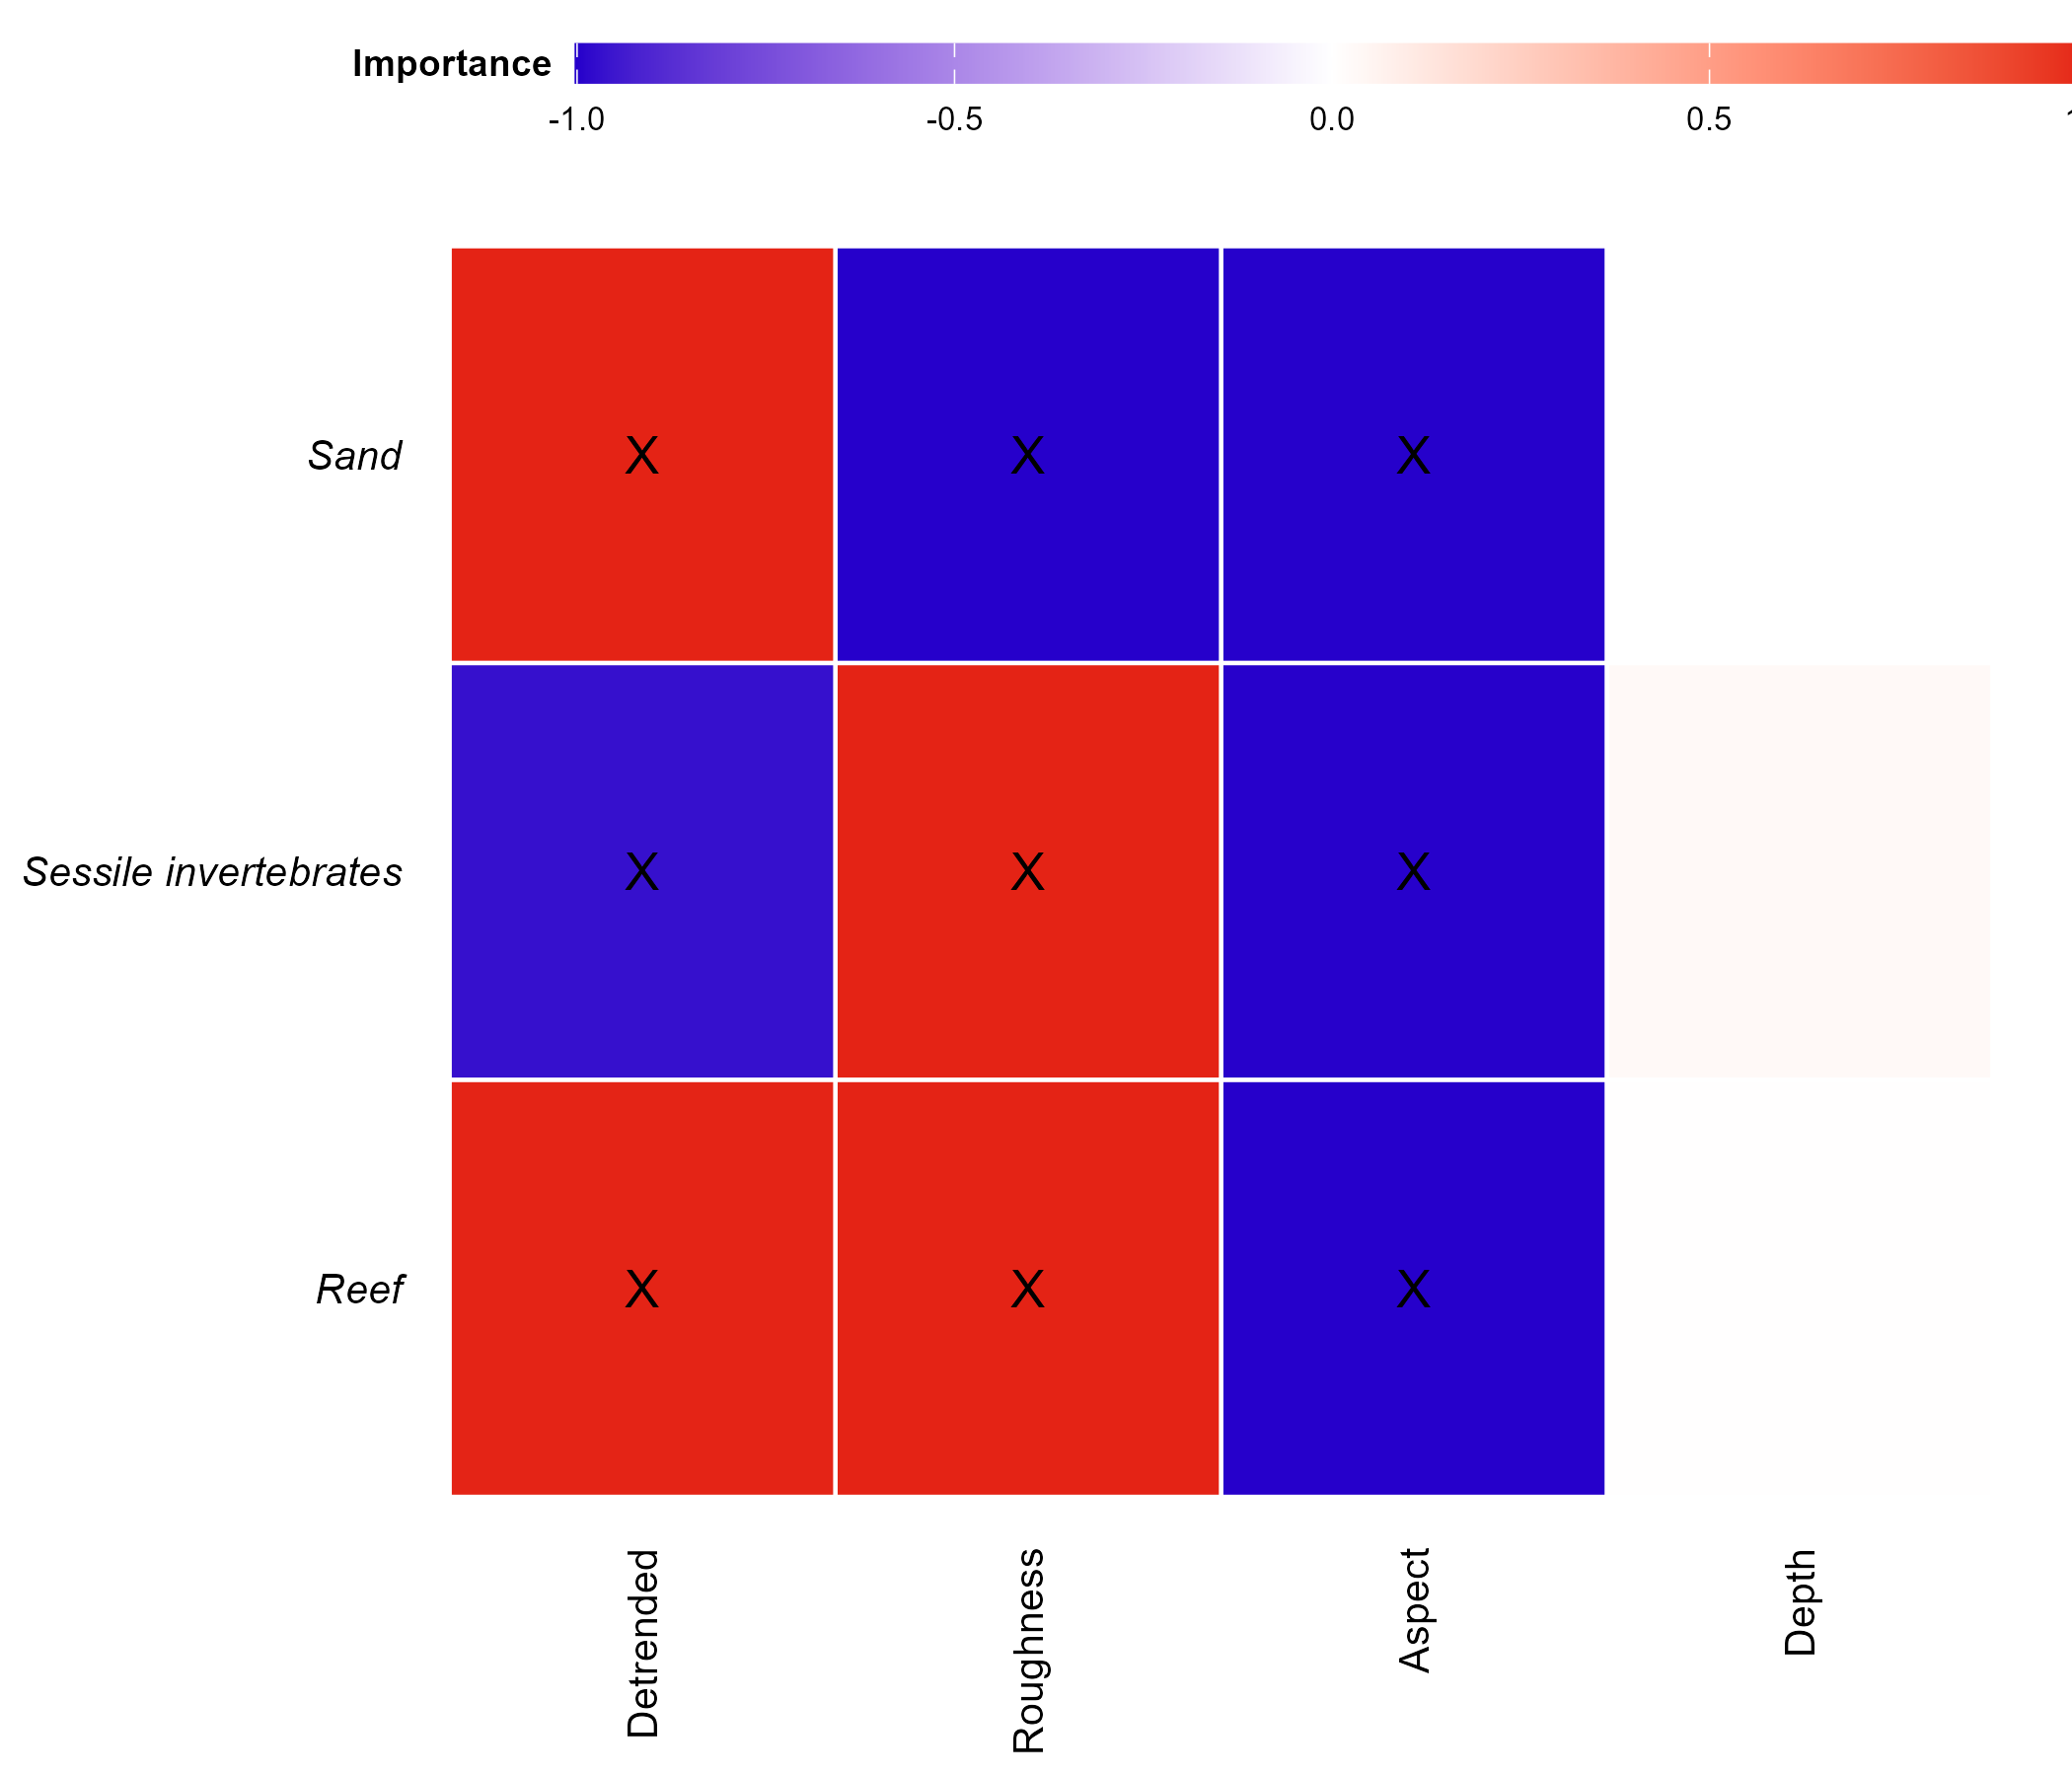
\includegraphics[width=0.85\linewidth,height=\textheight,keepaspectratio]{figures/BeagleAMP_habitat-importance.png}

}

\caption{Variable importance scores for predicting the probability of
occurrence of main habitat categories. Response variables included in
the most parsimonious top model are indicated (X), with the colour
gradient representing positive (red), zero (white) and negative (blue)
relationships. Aspect is a circular variable, so the direction of its
relationship should be read from the response curves rather than the
colour gradient.}

\end{figure}%

\newpage{}

\begin{figure}[H]

{\centering 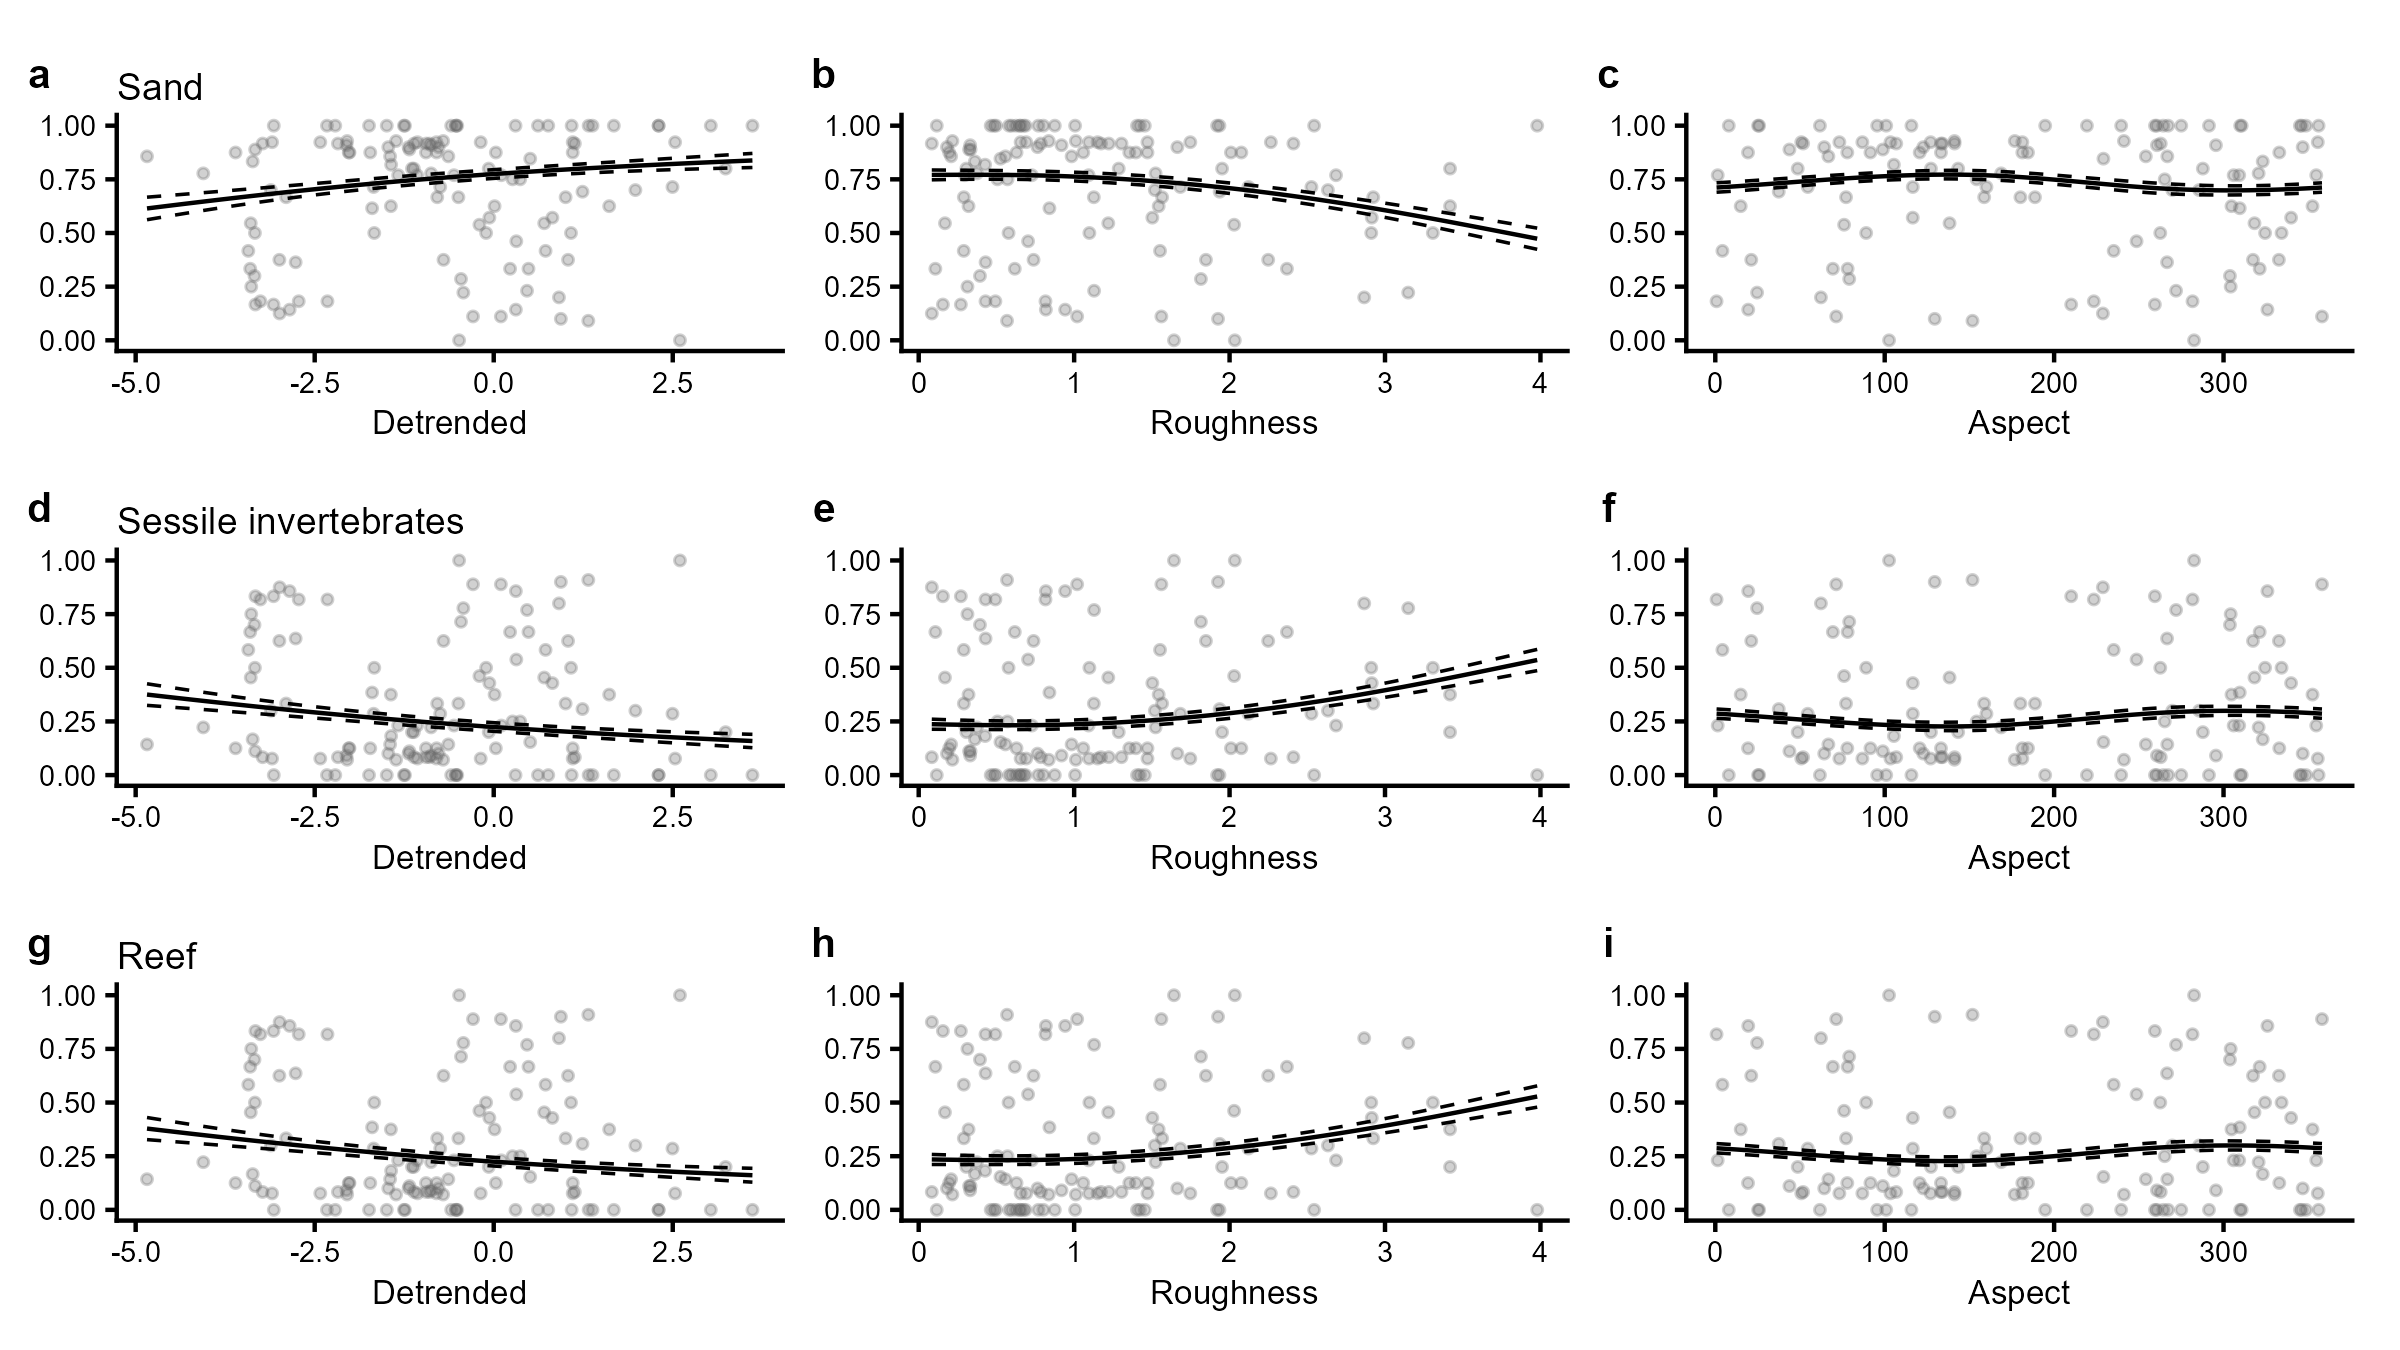
\includegraphics[width=1\linewidth,height=\textheight,keepaspectratio]{figures/BeagleAMP_habitat-response-curves_2018.png}

}

\caption{Plots of the most parsimonious model found to predict the
probability of occurrence of key habitat types. Individual panes display
the predicted relationships between model covariates and the probability
of occurrence of each habitat class. Solid lines represent predicted
Generalized Additive Model (GAM) fits with other variables held constant
at their mean value. Dashed lines represent upper and lower standard
error bounds around the prediction, and points represent the observed
data from all survey years.}

\end{figure}%

\begin{figure}[H]

{\centering 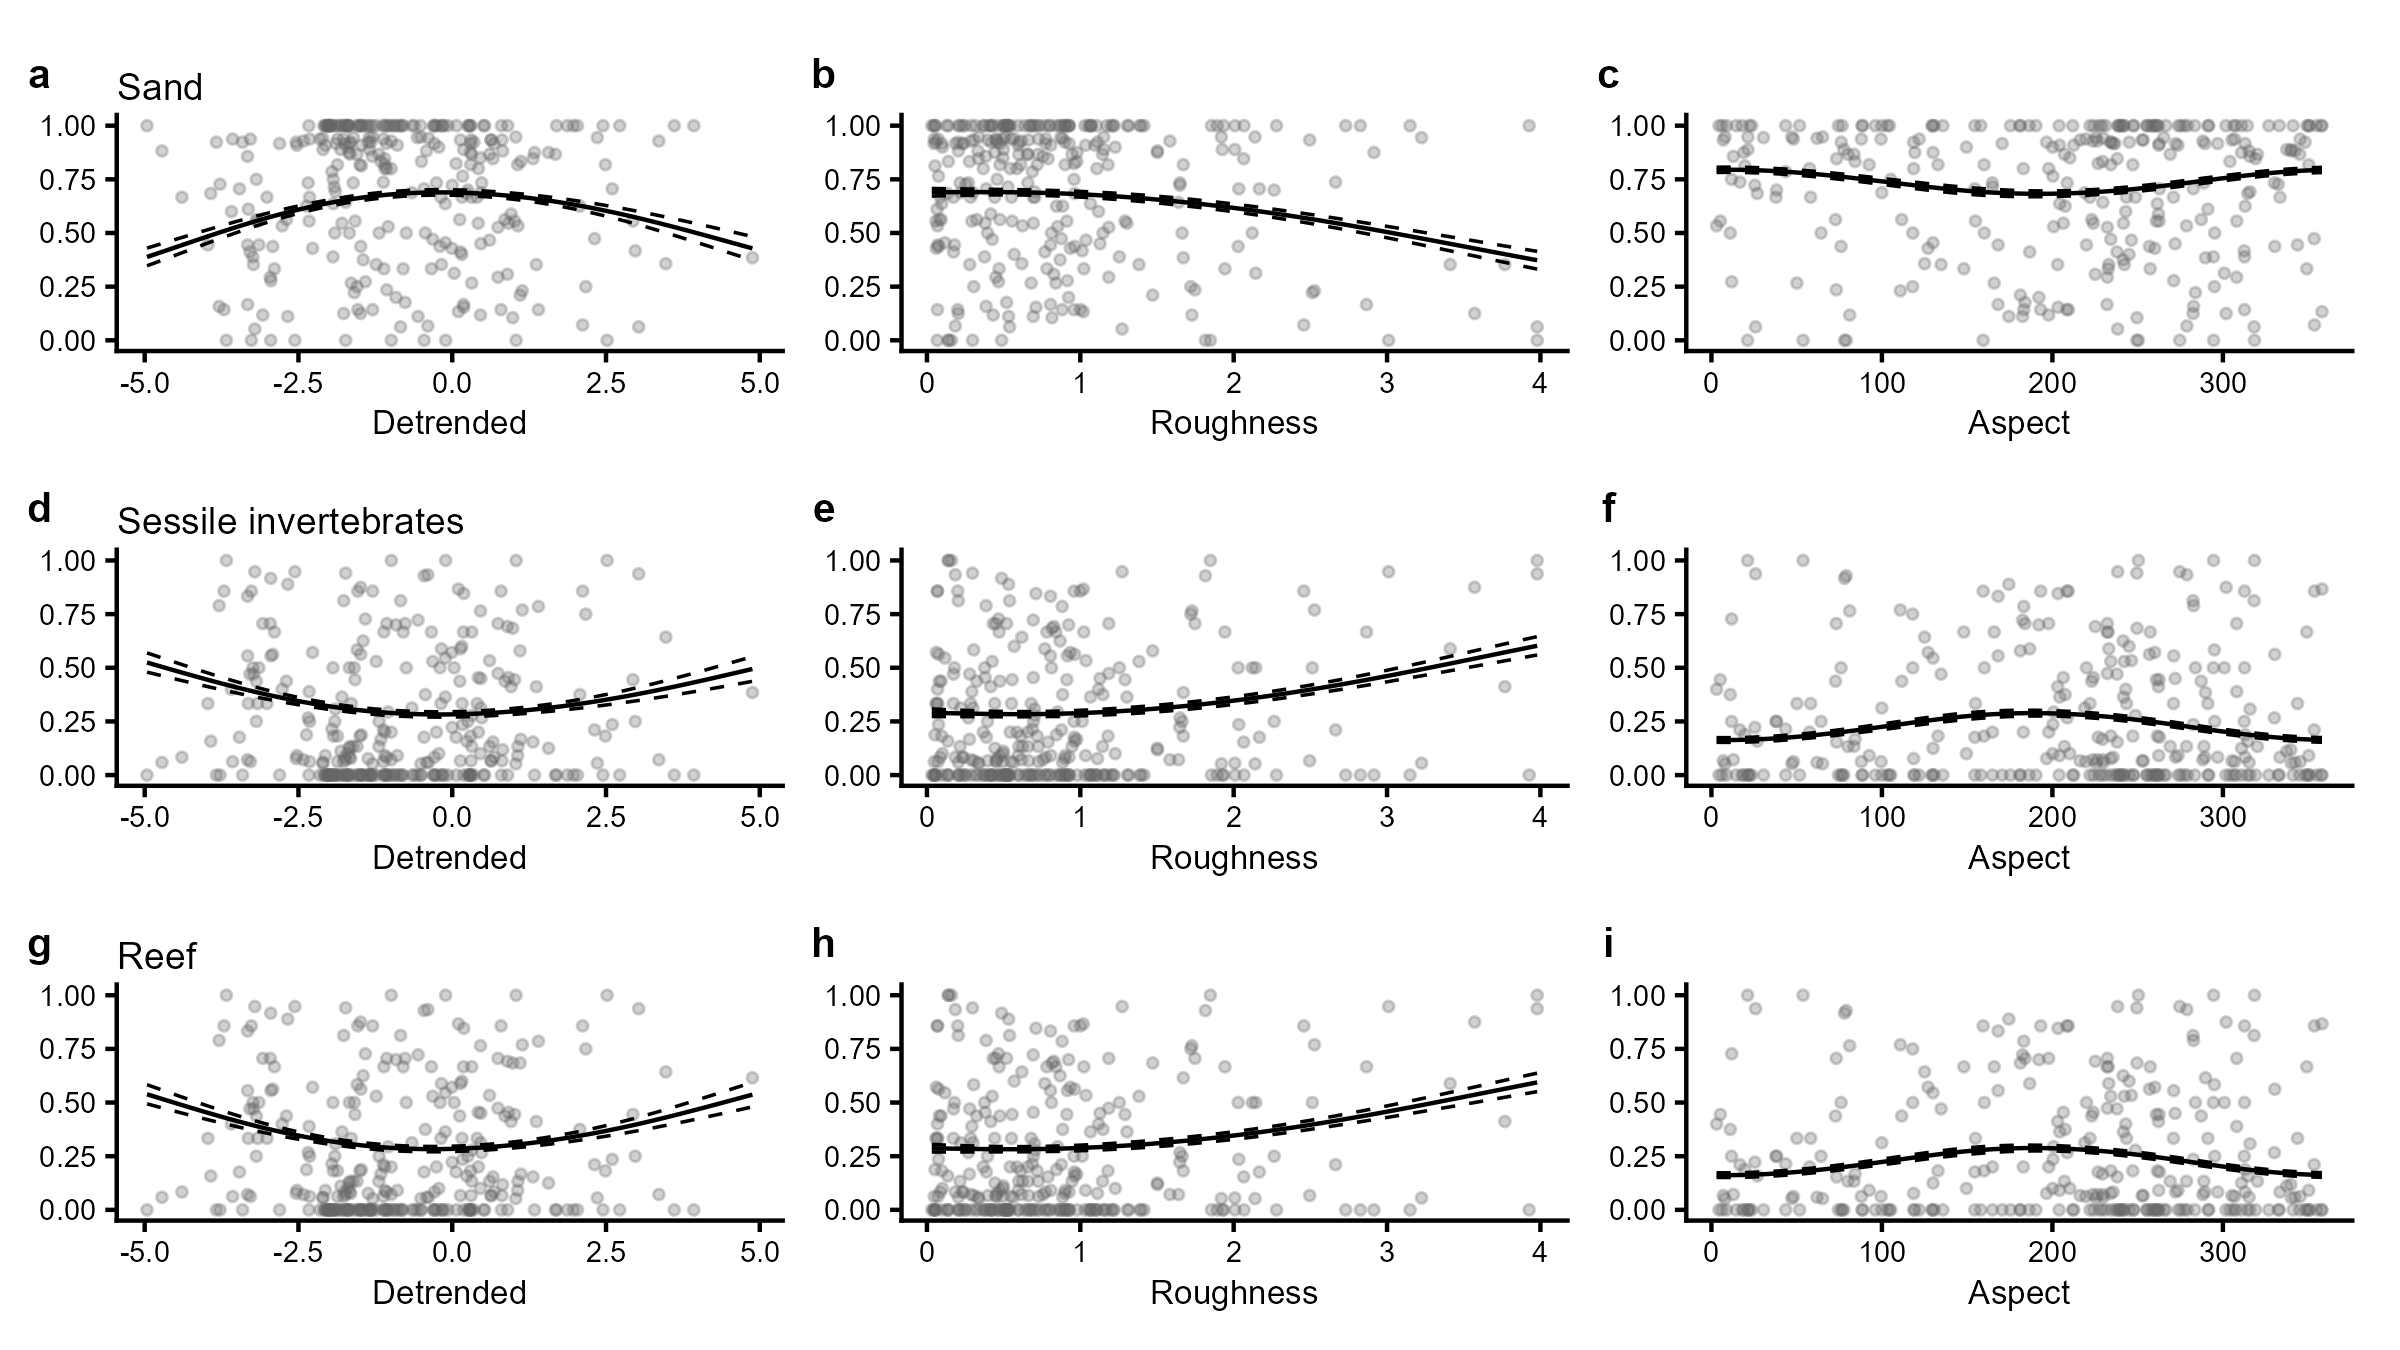
\includegraphics[width=1\linewidth,height=\textheight,keepaspectratio]{figures/BeagleAMP_habitat-response-curves_2025.png}

}

\caption{Plots of the most parsimonious model found to predict the
probability of occurrence of key habitat types. Individual panes display
the predicted relationships between model covariates and the probability
of occurrence of each habitat class. Solid lines represent predicted
Generalized Additive Model (GAM) fits with other variables held constant
at their mean value. Dashed lines represent upper and lower standard
error bounds around the prediction, and points represent the observed
data from all survey years.}

\end{figure}%

\newpage{}

\subsection{Demersal fish assemblage}\label{demersal-fish-assemblage}

\begingroup\fontsize{10}{12}\selectfont

\begin{longtable}[t]{>{\raggedright\arraybackslash}m{2.05cm}>{\centering\arraybackslash}m{4.392cm}>{\centering\arraybackslash}m{1.61cm}>{\centering\arraybackslash}m{1.61cm}>{\centering\arraybackslash}m{1.757cm}>{\centering\arraybackslash}m{1.757cm}>{\centering\arraybackslash}m{1.464cm}}

\caption{\label{tbl-c2-1}Demersal fish model selection results. Top
generalised additive models (GAMs) for predicting the species and
abundance distribution of metrics of interest from full subset analyses.
Differences between the lowest reported corrected Akaike Information
Criterion (\(\Delta\)AICc), AICc weight (\(\omega\)AICc), variance
explained (R\(^2\)) and effective degrees of freedom (EDF) are reported
for model comparison. Model selection was based on the best model
(fewest variables - shown in bold) within two units of the lowest AICc.
*Large Reef Fish Index representing the biomass of all fish greater than
20 cm (B20) has been adapted here for stereo-BRUV data by removing
sharks and rays.}

\tabularnewline

\toprule
\cellcolor{gray!25}{\textbf{Response}} & \cellcolor{gray!25}{\textbf{Model}} & \cellcolor{gray!25}{\textbf{$\Delta$ AICc}} & \cellcolor{gray!25}{\textbf{$\omega$ AICc}} & \cellcolor{gray!25}{\textbf{AICc}} & \cellcolor{gray!25}{\textbf{$R^2$}} & \cellcolor{gray!25}{\textbf{EDF}}\\
\midrule
\endfirsthead
\multicolumn{7}{@{}l}{\textit{(continued)}}\\
\toprule
\cellcolor{gray!25}{\textbf{Response}} & \cellcolor{gray!25}{\textbf{Model}} & \cellcolor{gray!25}{\textbf{$\Delta$ AICc}} & \cellcolor{gray!25}{\textbf{$\omega$ AICc}} & \cellcolor{gray!25}{\textbf{AICc}} & \cellcolor{gray!25}{\textbf{$R^2$}} & \cellcolor{gray!25}{\textbf{EDF}}\\
\midrule
\endhead

\endfoot
\bottomrule
\endlastfoot
 & detrended+reef+year+status+geoscience_aspect.by.year+geoscience_depth.by.year & 0 & 0.141 & 2195.32 & 0.28899 & 9.91\\
 & detrended+year+status+geoscience_aspect.by.year+geoscience_depth.by.year+reef.by.year & 0.163 & 0.13 & 2195.48 & 0.29303 & 11.20\\
 & reef+year+status+geoscience_aspect.by.year+geoscience_depth.by.year+geoscience_detrended.by.year & 1.189 & 0.078 & 2196.51 & 0.29024 & 10.86\\
\multirow{1}{=}{Species richness} & detrended+reef+year+status+geoscience_depth.by.year & 1.19 & 0.078 & 2196.51 & 0.28062 & 7.57\\
 & year+status+geoscience_aspect.by.year+geoscience_depth.by.year+geoscience_detrended.by.year+reef.by.year & 1.215 & 0.077 & 2196.53 & 0.29436 & 12.12\\
 & detrended+aspect+reef+year+status+geoscience_depth.by.year & 1.754 & 0.059 & 2197.07 & 0.28262 & 8.57\\
 & detrended+year+status+geoscience_depth.by.year+reef.by.year & 1.901 & 0.054 & 2197.22 & 0.28374 & 8.82\\
\noalign{\arrayrulecolor{gray}}\cdashline{1-7}\noalign{\arrayrulecolor{black}}
 & year+status+geoscience_depth.by.year+geoscience_detrended.by.year+reef.by.year & 0 & 0.115 & 3602.62 & 0.43434 & 11.31\\
 & year+status+geoscience_aspect.by.year+geoscience_depth.by.year+geoscience_detrended.by.year+reef.by.year & 0.005 & 0.114 & 3602.62 & 0.43435 & 13.31\\
 & aspect+year+status+geoscience_depth.by.year+geoscience_detrended.by.year+reef.by.year & 0.039 & 0.112 & 3602.66 & 0.43439 & 12.31\\
 & year+status+geoscience_depth.by.year+reef.by.year & 0.423 & 0.093 & 3603.04 & 0.42631 & 8.65\\
\multirow{1}{=}{Total abundance} & year+status+geoscience_aspect.by.year+geoscience_depth.by.year+reef.by.year & 0.425 & 0.093 & 3603.04 & 0.42631 & 10.65\\
 & aspect+year+status+geoscience_depth.by.year+reef.by.year & 0.442 & 0.092 & 3603.06 & 0.42633 & 9.65\\
 & year+status+geoscience_depth.by.year+geoscience_roughness.by.year+reef.by.year & 1.379 & 0.057 & 3604.00 & 0.43485 & 11.79\\
 & year+status+geoscience_aspect.by.year+geoscience_depth.by.year+geoscience_roughness.by.year+reef.by.year & 1.393 & 0.057 & 3604.01 & 0.43486 & 13.79\\
 & aspect+year+status+geoscience_depth.by.year+geoscience_roughness.by.year+reef.by.year & 1.399 & 0.057 & 3604.02 & 0.43487 & 12.79\\
\noalign{\arrayrulecolor{gray}}\cdashline{1-7}\noalign{\arrayrulecolor{black}}
 & aspect+reef+year+status+geoscience_depth.by.year+geoscience_roughness.by.year & 0 & 0.182 & 3266.53 & 0.35509 & 10.94\\
 & roughness+aspect+year+status+geoscience_depth.by.year+reef.by.year & 0.422 & 0.148 & 3266.96 & 0.35748 & 11.52\\
\multirow{1}{=}{Large Reef Fish Index*} & aspect+year+status+geoscience_depth.by.year+geoscience_detrended.by.year+reef.by.year & 0.919 & 0.115 & 3267.45 & 0.36404 & 13.06\\
 & aspect+year+status+geoscience_depth.by.year+geoscience_roughness.by.year+reef.by.year & 0.944 & 0.114 & 3267.48 & 0.3615 & 12.39\\
 & roughness+aspect+reef+year+status+geoscience_depth.by.year & 1.052 & 0.108 & 3267.59 & 0.35157 & 10.54\\
 & aspect+reef+year+status+geoscience_depth.by.year+geoscience_detrended.by.year & 1.95 & 0.069 & 3268.48 & 0.3571 & 12.17\\
\noalign{\arrayrulecolor{gray}}\cdashline{1-7}\noalign{\arrayrulecolor{black}}
\multirow{1}{=}{Reef Fish Thermal Index} & year+status+geoscience_aspect.by.year+geoscience_depth.by.year+reef.by.year & 0 & 0.16 & 850.07 & 0.2557 & 10.70\\
 & aspect+year+status+geoscience_depth.by.year+reef.by.year & 0.056 & 0.156 & 850.13 & 0.25586 & 9.77\\*

\end{longtable}

\endgroup{}

\begin{figure}[H]

{\centering 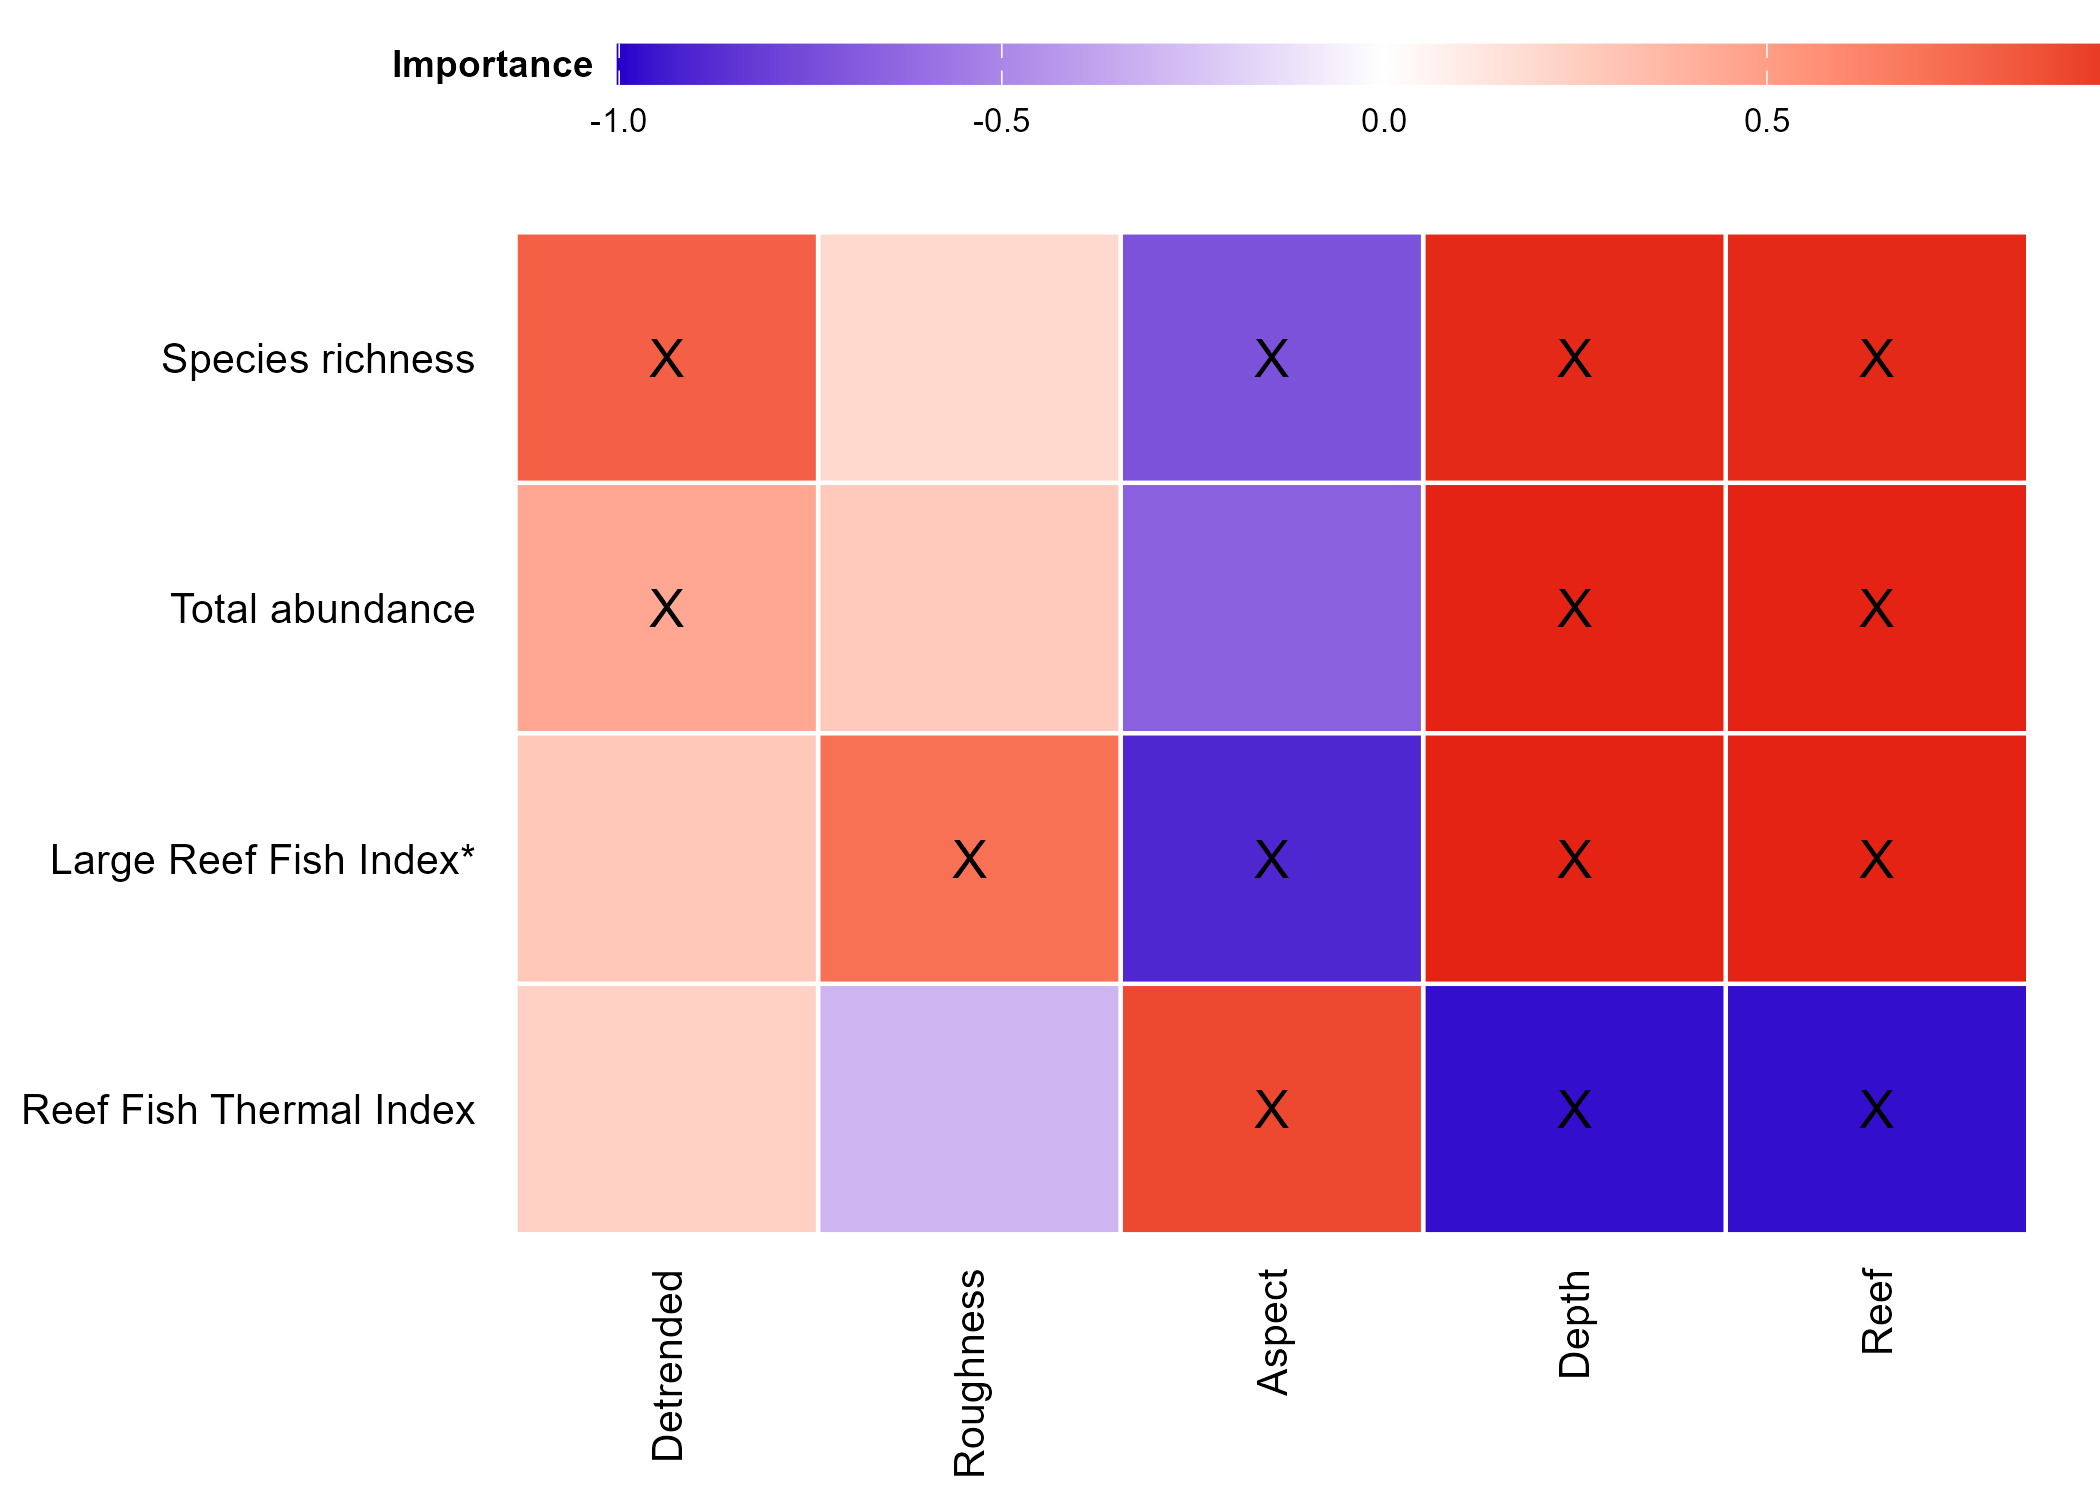
\includegraphics[width=0.85\linewidth,height=\textheight,keepaspectratio]{figures/BeagleAMP_fish-importance.png}

}

\caption{Variable importance scores for predicting the probability of
demersal fish metrics. Response variables included in the most
parsimonious top model are indicated (X), with the colour gradient
representing positive (red), zero (white) and negative (blue)
relationships. Aspect is a circular variable, so the direction of its
relationship should be read from the response curves rather than the
colour gradient. *Large Reef Fish Index representing the biomass of all
fish greater than 20 cm (B20) has been adapted here for stereo-BRUV data
by removing sharks and rays.}

\end{figure}%

\newpage{}

\begin{figure}[H]

{\centering 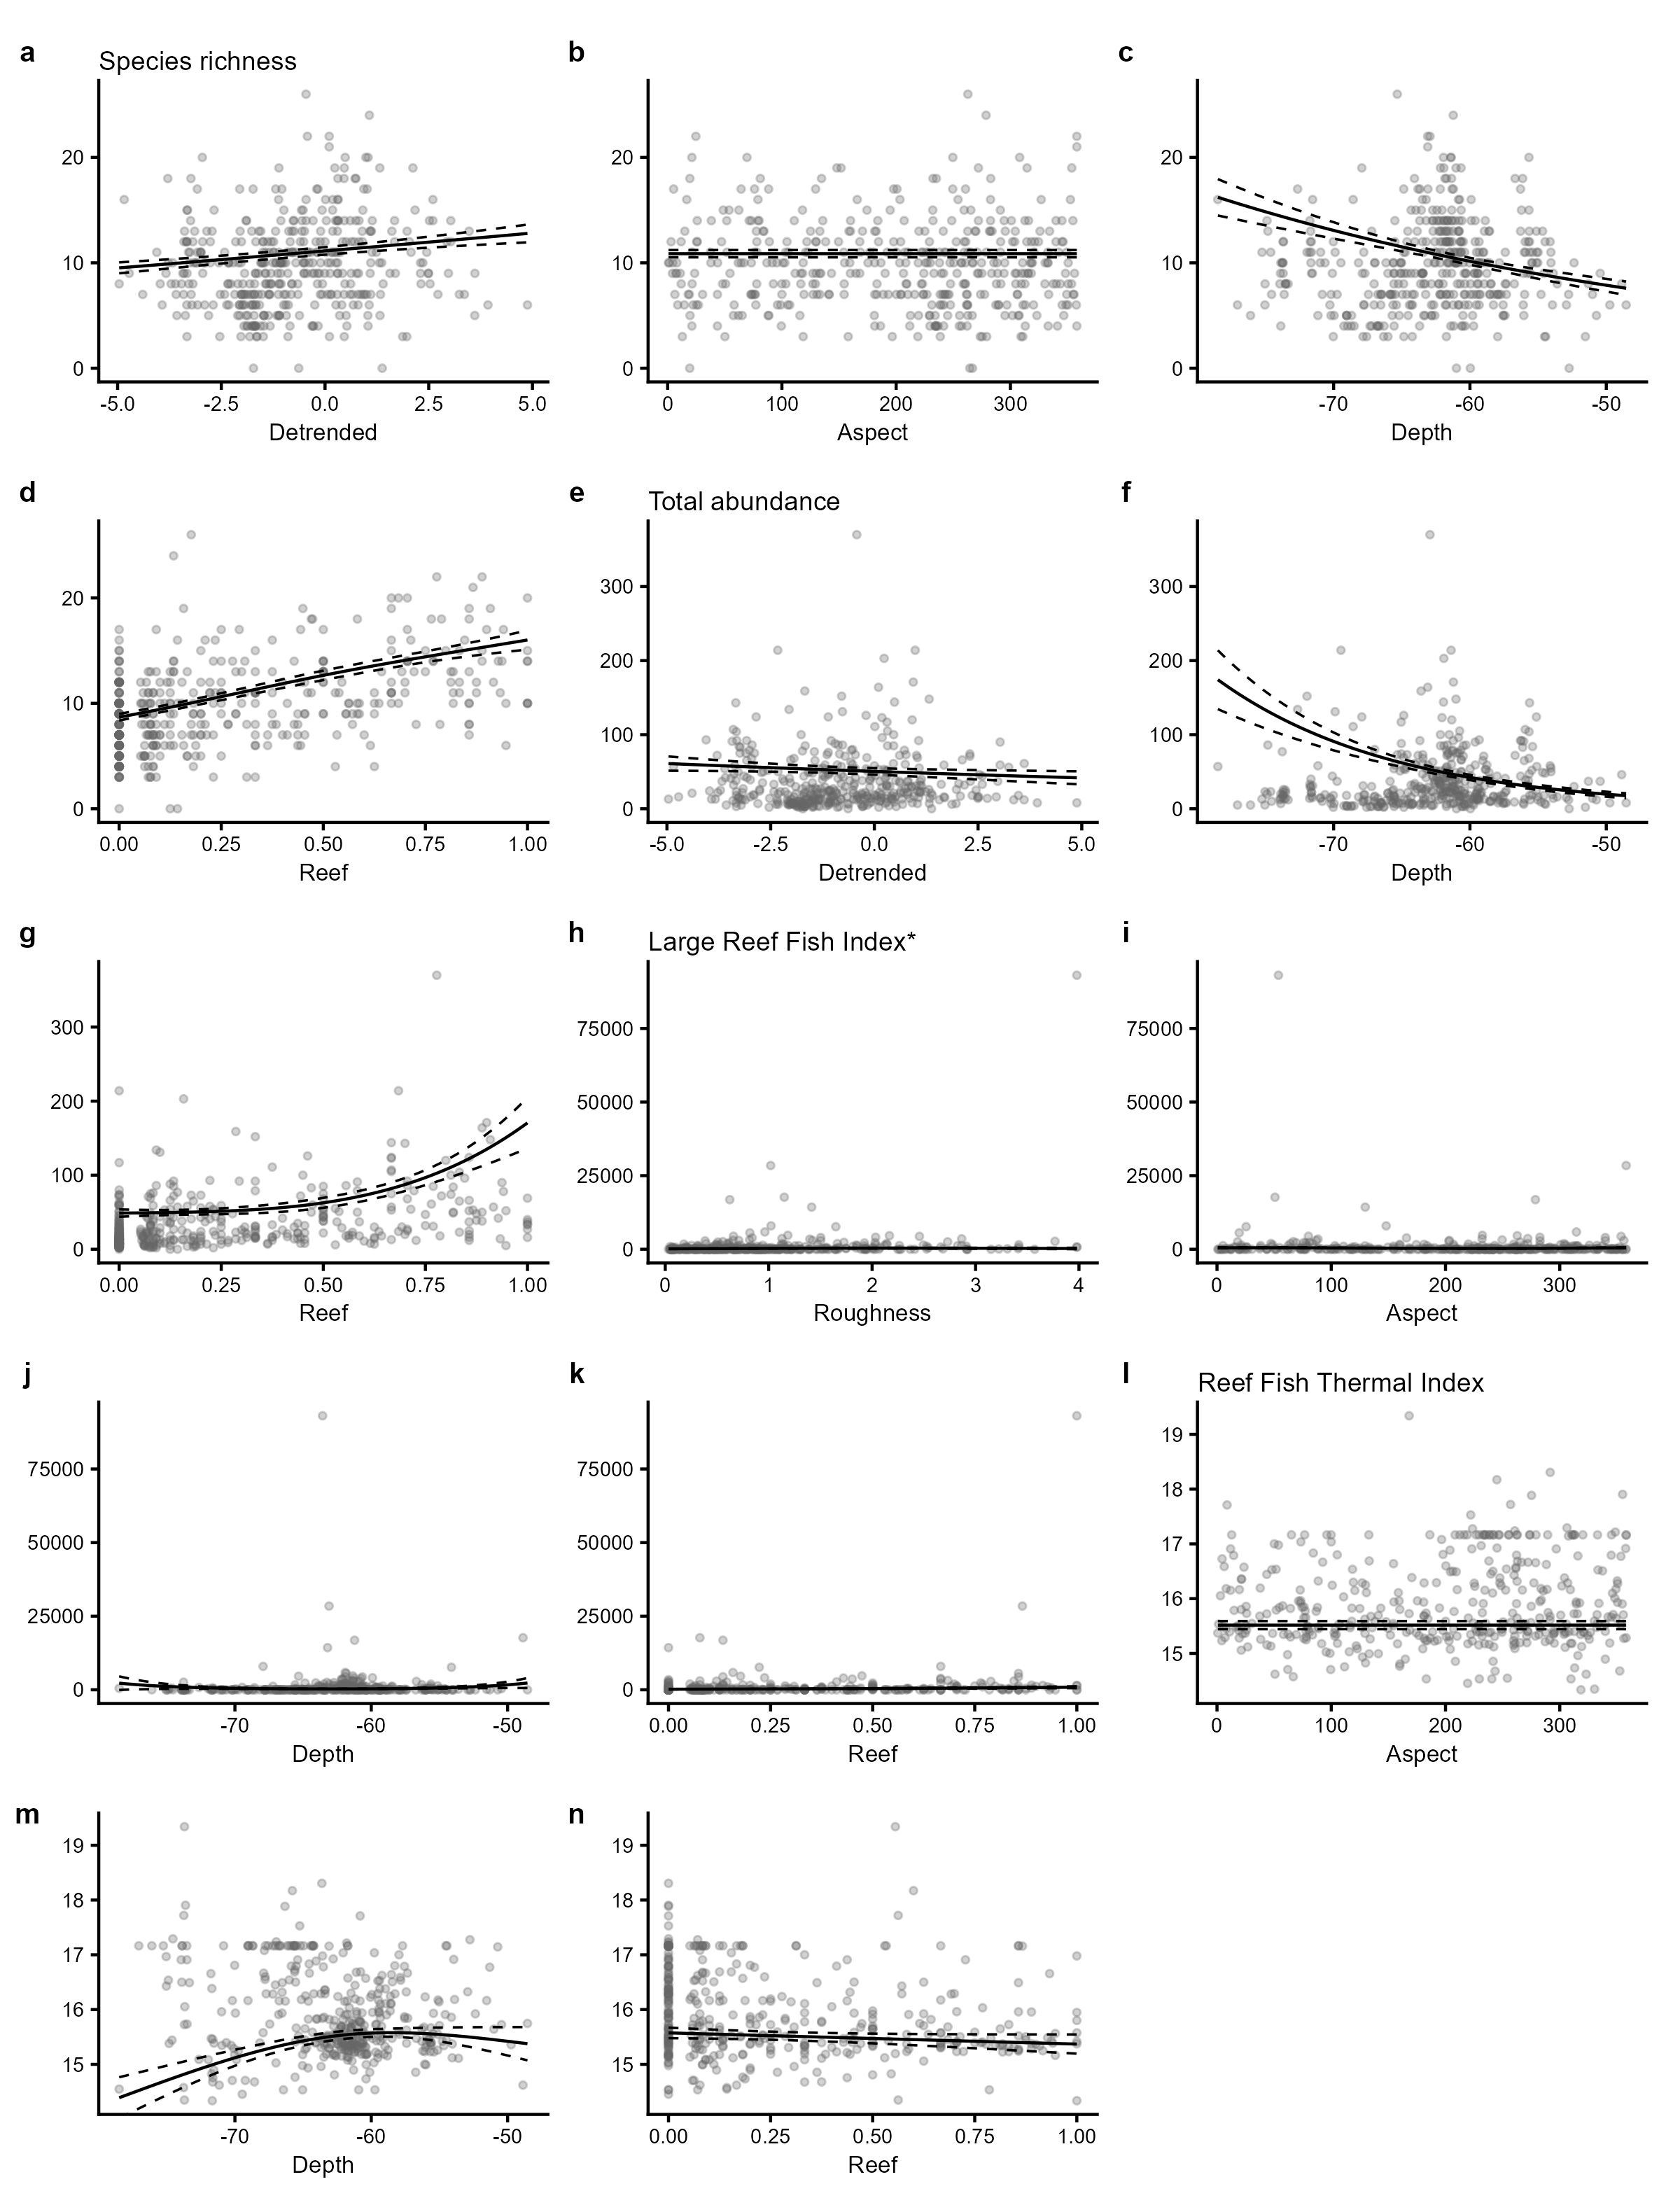
\includegraphics[width=0.8\linewidth,height=\textheight,keepaspectratio]{figures/BeagleAMP_fish-response-curves_2018.png}

}

\caption{Plots of the best model found to predict the probability of
occurrence of key fish groups. Individual panes display the predicted
relationships between model covariates and each demersal fish metric.
Solid lines represent predicted Generalized Additive Model (GAM) fits
with other variables held constant at their mean value, with year held
at 2018 and zone status held at areas open to fishing. Dashed lines
represent upper and lower standard error bounds around the prediction,
and points represent the observed data from all survey years and zones.
*Large Reef Fish Index representing the biomass of all fish greater than
20 cm (B20) has been adapted here for stereo-BRUV data by removing
sharks and rays.}

\end{figure}%

\begin{figure}[H]

{\centering 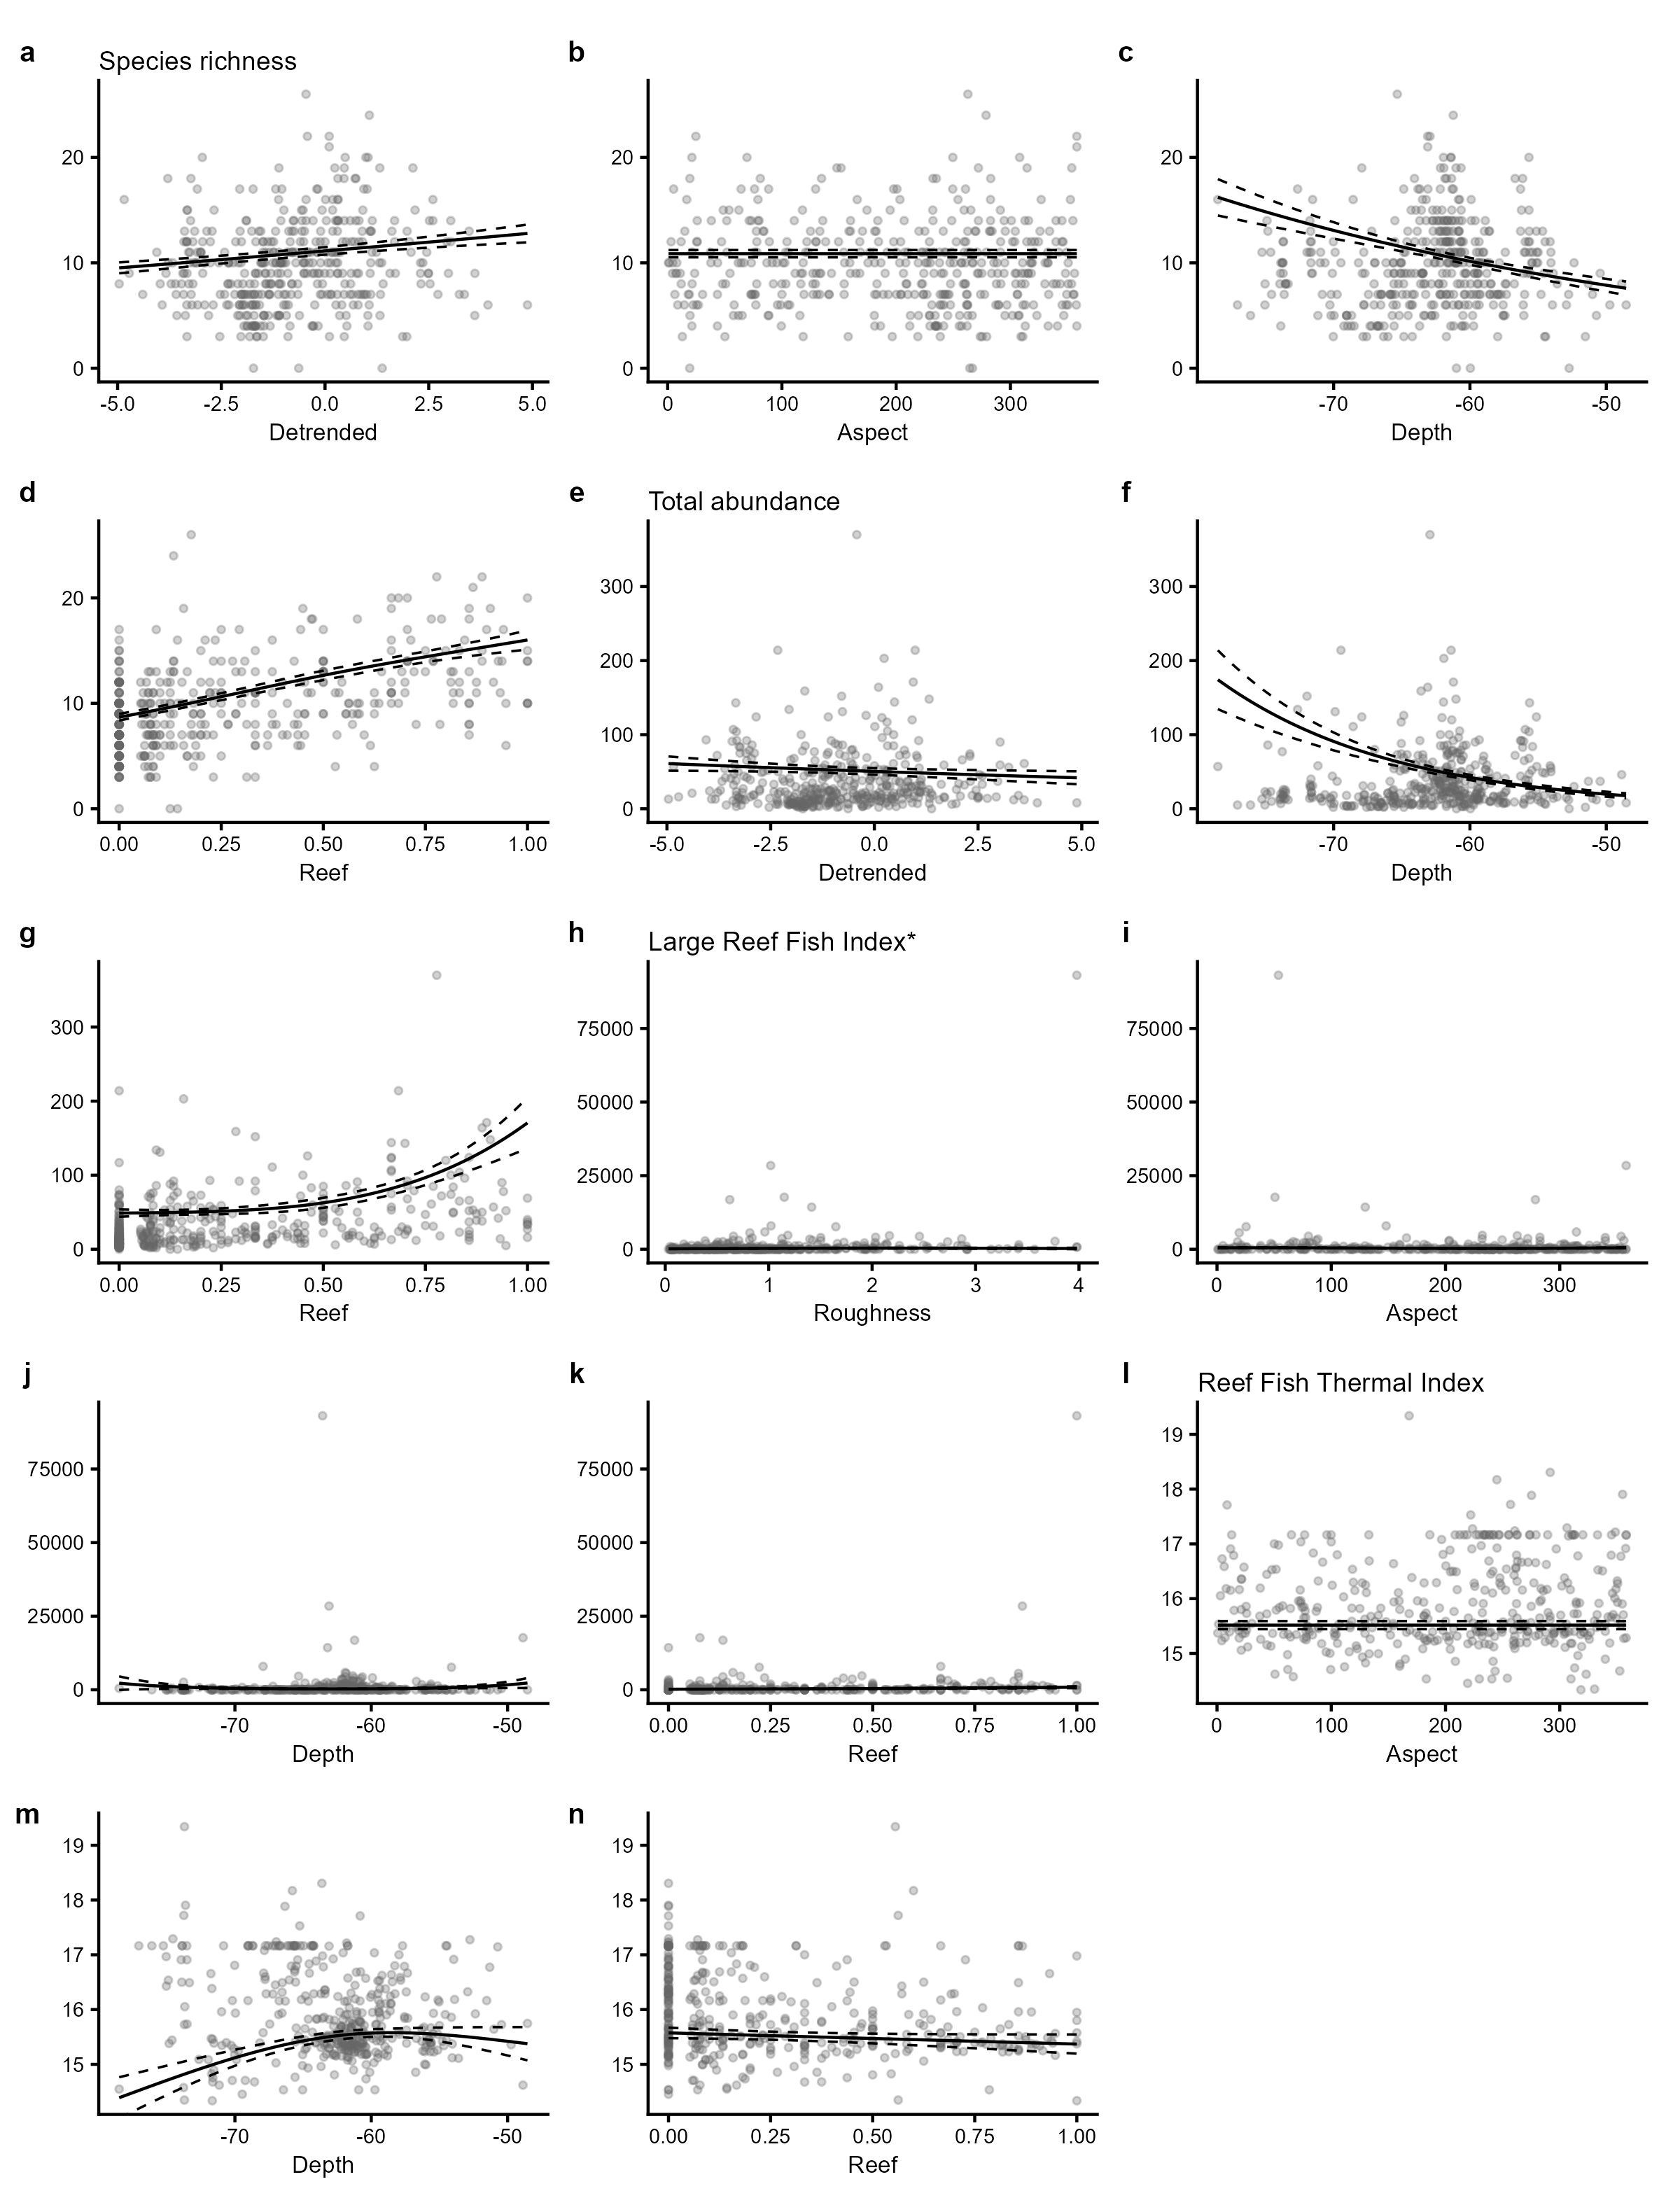
\includegraphics[width=0.8\linewidth,height=\textheight,keepaspectratio]{figures/BeagleAMP_fish-response-curves_2018.png}

}

\caption{Plots of the best model found to predict the probability of
occurrence of key fish groups. Individual panes display the predicted
relationships between model covariates and each demersal fish metric.
Solid lines represent predicted Generalized Additive Model (GAM) fits
with other variables held constant at their mean value, with year held
at 2018 and zone status held at areas open to fishing. Dashed lines
represent upper and lower standard error bounds around the prediction,
and points represent the observed data from all survey years and zones.
*Large Reef Fish Index representing the biomass of all fish greater than
20 cm (B20) has been adapted here for stereo-BRUV data by removing
sharks and rays.}

\end{figure}%

\newpage{}

\subsection{Significance of year and zone
status}\label{significance-of-year-and-zone-status}

\begingroup\fontsize{10}{12}\selectfont

\begin{longtable}[t]{llcccc}

\caption{\label{tbl-c3-1}Significance of the year and zone status terms
in each demersal fish GAMM. Estimate, standard error (SE), test
statistic and p-value are taken from the parametric coefficient table of
each model summary, one row per factor-level contrast (e.g.~a survey
year against the reference year, or No-Take against Fished).}

\tabularnewline

\toprule
\cellcolor{gray!25}{\textbf{Response}} & \cellcolor{gray!25}{\textbf{Term}} & \cellcolor{gray!25}{\textbf{Estimate}} & \cellcolor{gray!25}{\textbf{SE}} & \cellcolor{gray!25}{\textbf{Statistic}} & \cellcolor{gray!25}{\textbf{p-value}}\\
\midrule
\endfirsthead
\multicolumn{6}{@{}l}{\textit{(continued)}}\\
\toprule
\cellcolor{gray!25}{\textbf{Response}} & \cellcolor{gray!25}{\textbf{Term}} & \cellcolor{gray!25}{\textbf{Estimate}} & \cellcolor{gray!25}{\textbf{SE}} & \cellcolor{gray!25}{\textbf{Statistic}} & \cellcolor{gray!25}{\textbf{p-value}}\\
\midrule
\endhead

\endfoot
\bottomrule
\endlastfoot
Species richness & Zone status: No-Take vs Fished & -0.108 & 0.095 & -1.135 & 0.256\\
 & Year: 2025 vs 2018 & -0.119 & 0.035 & -3.414 & <0.001\\
Total abundance & Zone status: No-Take vs Fished & 0.232 & 0.198 & 1.171 & 0.242\\
 & Year: 2025 vs 2018 & -0.886 & 0.074 & -11.906 & <0.001\\
Large Reef Fish Index* & Zone status: No-Take vs Fished & -0.921 & 0.630 & -1.462 & 0.145\\
 & Year: 2025 vs 2018 & 0.338 & 0.242 & 1.396 & 0.164\\
Reef Fish Thermal Index & Zone status: No-Take vs Fished & 0.158 & 0.192 & 0.823 & 0.411\\
 & Year: 2025 vs 2018 & 0.592 & 0.078 & 7.596 & <0.001\\*

\end{longtable}

\endgroup{}

\begin{table}

\caption{\label{tbl-c3-2}Zone status test for each demersal fish metric,
laid out by survey year. Zone status (No-Take vs Fished) is fitted as a
single term across all years (no year by status interaction), so the
status estimate, SE and p-value are the same in every row for a given
metric; predicted values and their SE are shown per year, with other
model covariates held at their mean.}

\centering{

\centering\begingroup\fontsize{10}{12}\selectfont

\resizebox{\ifdim\width>\linewidth\linewidth\else\width\fi}{!}{
\begin{tabular}[t]{lcccccccc}
\toprule
\cellcolor{gray!25}{\textbf{Response}} & \cellcolor{gray!25}{\textbf{Year}} & \cellcolor{gray!25}{\textbf{Fished (predicted)}} & \cellcolor{gray!25}{\textbf{Fished (SE)}} & \cellcolor{gray!25}{\textbf{No-Take (predicted)}} & \cellcolor{gray!25}{\textbf{No-Take (SE)}} & \cellcolor{gray!25}{\textbf{Status estimate}} & \cellcolor{gray!25}{\textbf{Status SE}} & \cellcolor{gray!25}{\textbf{Status p-value}}\\
\midrule
Species richness & 2018 & 10.865 & 0.345 & 9.755 & 0.965 & -0.108 & 0.095 & 0.256\\
 & 2025 & 9.813 & 0.340 & 8.810 & 0.834 & -0.108 & 0.095 & 0.256\\
Total abundance & 2018 & 51.985 & 4.250 & 65.535 & 14.028 & 0.232 & 0.198 & 0.242\\
 & 2025 & 33.213 & 2.495 & 41.870 & 8.326 & 0.232 & 0.198 & 0.242\\
Large Reef Fish Index* & 2018 & 298.291 & 85.699 & 118.813 & 81.900 & -0.921 & 0.630 & 0.145\\
 & 2025 & 873.972 & 163.249 & 348.114 & 218.827 & -0.921 & 0.630 & 0.145\\
Reef Fish Thermal Index & 2018 & 15.516 & 0.074 & 15.674 & 0.205 & 0.158 & 0.192 & 0.411\\
 & 2025 & 15.845 & 0.078 & 16.003 & 0.191 & 0.158 & 0.192 & 0.411\\
\bottomrule
\end{tabular}}
\endgroup{}

}

\end{table}%




\end{document}
